\documentclass[12pt,french]{article} %ajouter draft pour voir débordement
\usepackage[utf8]{inputenc}
\usepackage[T1]{fontenc}
\usepackage{lmodern}
%règles mes marges et format papier
\usepackage[a4paper,hmargin=2cm,vmargin=2cm]{geometry} %modif marge et formet
\usepackage{amsmath, amssymb, amsthm}
\usepackage{fancyhdr} %pour les entêtes et bas de page
\usepackage{lastpage} %pour numéroter les pages charge la derniere page
\usepackage{graphicx} %pour inclure des img
\usepackage{dsfont}
\usepackage{float} %pour le placement des figures
\usepackage{hyperref} %pour mettre des liens hypertext
\usepackage{calc} %permet de calculer les marges pour encadrer les textes
\usepackage{color, xcolor} %gère les couleurs
\usepackage{babel}
\usepackage{listings} %pour afficher le code annexe

%pour afficher le code de manière esthétique
\lstset{
  aboveskip=3mm,
  belowskip=-2mm,
  backgroundcolor=\color{white},
  basicstyle=\footnotesize,
  breakatwhitespace=false,
  breaklines=true,
  captionpos=b,
  commentstyle=\color{red},
  deletekeywords={...},
  escapeinside={\%*}{*)},
  extendedchars=true,
  framexleftmargin=16pt,
  framextopmargin=3pt,
  framexbottommargin=6pt,
  frame=tb,
  keepspaces=true,
  keywordstyle=\color{blue},
  language=C,
  literate=
  {²}{{\textsuperscript{2}}}1 {⁴}{{\textsuperscript{4}}}1
  {⁶}{{\textsuperscript{6}}}1
  {⁸}{{\textsuperscript{8}}}1
  {€}{{\euro{}}}1 {é}{{\'e}}1 {è}{{\`{e}}}1 {ê}{{\^{e}}}1 {ë}{{\¨{e}}}1
  {É}{{\'{E}}}1 {Ê}{{\^{E}}}1 {û}{{\^{u}}}1 {ù}{{\`{u}}}1 {â}{{\^{a}}}1
  {à}{{\`{a}}}1 {á}{{\'{a}}}1 {ã}{{\~{a}}}1 {Á}{{\'{A}}}1 {Â}{{\^{A}}}1
  {Ã}{{\~{A}}}1 {ç}{{\c{c}}}1 {Ç}{{\c{C}}}1 {õ}{{\~{o}}}1 {ó}{{\'{o}}}1 
  {ô}{{\^{o}}}1 {Õ}{{\~{O}}}1 {Ó}{{\'{O}}}1 {Ô}{{\^{O}}}1 {î}{{\^{i}}}1
  {Î}{{\^{I}}}1 {í}{{\'{i}}}1 {Í}{{\~{Í}}}1,
  morekeywords={*,...},
  numbers=left,
  numbersep=10pt,
  numberstyle=\tiny\color{black},
  rulecolor=\color{black},
  showspaces=false,
  showstringspaces=false,
  showtabs=false,
  stepnumber=1,
  stringstyle=\color{gray},
  tabsize=4,
}
%%%%%

%Personalisation En tête
\pagestyle{fancy}
\renewcommand\headrulewidth{1pt}
%permet d'aumenter tailler header pour mettre image (31pt ici)
\setlength{\headheight}{31pt}
\fancyhead[L]{Simulation - F2}
\fancyhead[C]{
\includegraphics[scale=0.2]{header.png}}
\fancyhead[R]{Lab \#2 - Generation of \\ Random Variates}
\renewcommand\footrulewidth{1pt}
\fancyfoot[L]{BALLEJOS Lilian}
\fancyfoot[C]{\thepage/\pageref{LastPage}}
\fancyfoot[R]{2021/2022}
%Fin personalisation En Tête


\begin{document}

\begin{titlepage} %page d'acceuil

  
  
\includegraphics[scale=0.6]{isima.png}
  \hspace*{\stretch{1}}%espace horizontal entre les 2 images
  
\includegraphics[scale=0.25]{deco.png}
  
  \vspace*{2.5cm} %espace de 2.5cm en dessous des images
  
  \begin{center}\huge
    \textbf{Rapport TP Simulation} 
    
    \textbf{Lab \#2 - Generation of Random Variates}
  \end{center}
  
  \hrule %trait horizontal
  
  \begin{center}
    \Large BALLEJOS Lilian
    
    \large
    ISIMA INP Deuxième année
    
    Spécialité F2
    
    Année Universitaire 2021/2022
  \end{center}
  
  \begin{center}
    %créer une boite ou mettre l'image qui fait la largeur de la page
    \makebox[\textwidth]{
\includegraphics[width=\paperwidth]{garde.png}}
  \end{center}
  
  \vspace*{2cm} 
  
  \begin{flushright}\footnotesize %a droite
    Enseignant référant: Mr David HILL
    
    Date du rendu: 17 octobre 2022
    
    Date de la dernière modification: \today 
    %permet d'afficher la date ou je code actuellement (\today)
    
  \end{flushright}
  
  \begin{flushleft}\small %a gauche
    \textbf{ISIMA INP}
    \footnotesize
    
    1 rue de la Chebarde - TSA 60125 - CS 60026 - 63178 Aubière CEDEX
    
    Tel: 04 73 40 50 00
    
    Site web: \href{https://www.isima.fr/}{isima.fr}\newline	
  \end{flushleft}
\end{titlepage}	


%Ma table des Matières !
%permet de renommer 'table des matières' en sommaire
\renewcommand{\contentsname}{Table des Matières}
\normalsize\tableofcontents %place la table des matières

\bigskip

\section*{Introduction}

Nous allons dans ce TP nous intéresser  à la génération de nombre aléatoire uniforme entre [0 , 1] en s'appuyant sur les fonctions de génération de Matsumoto que vous pouvez retrouver \href{http://www.math.sci.hiroshima-u.ac.jp/m-mat/eindex.html}{\underline{ici}}.

Nous allons voir qu'à partir de ces fonctions de génération nous pouvons approcher de manière empirique de nombreuses sorties aléatoire de loi connue (loi normale, loi exponentielle ...).

\subsection*{Quelques remarques sur le fichier .c}

Les commentaires \textbf{/**/} sont voués à être supprimés Ils sont ici pour rendre l'exécution du main plus lisible et ne pas biaiser les tirages aléatoires en enchainant des tirages.

\bigskip

La compilation s'effectue comme ceci : \textbf{gcc -Wall -Wextra -g -o tp2\_ballejos tp2\_ballejos.c -lm}

\bigskip

Il faut bien penser à créer le répertoire \textbf{"sorti"} si vous souhaitez voir les sorties de certaines fonctions dans des fichiers.


\newpage

\section{Exercice 1: Test des sorties des fonctions MT}

Nous allons commencez par vérifier si le code que nous utilisons est portable. Pour cela nous possédons les sorties de code effectuer par Matsumoto sur sa machine qui se trouve dans le fichier \textbf{"mt19937ar.out"}.

J'ai donc appelé le programme cette fois ci sur ma machine afin de tester si les sorties sont les même. Pour cela j'ai récupéré les sorties du programme à l'exécution dans un fichier \textbf{test.out} comme ceci:

\begin{lstlisting}
	./mt19937ar > test.out
\end{lstlisting}

\bigskip

J'ai ensuite comparé le contenu des deux fichiers avec la commande bash \textbf{diff} qui affiche toutes les différences présentes entre deux fichiers.

\begin{lstlisting}
	diff test.out mt19937ar.out
\end{lstlisting}

\bigskip

En l'occurrence, la sortie de mon diff est ici vide ce qui implique que j'ai obtenu les mêmes sorties que Matsumoto et que le code est bien portable sur différentes machines !


\section{Exercice 2: Tirage aléatoire uniforme sur un intervalle}

Nous allons maintenant commencer à jouer avec les fonctions MT en tirant des nombres aléatoires uniformément dans un intervalle voulu. Pour cela nous utilisons (et cela jusqu'à la fin du TP) la fonction \textbf{genrand\_real2()} qui génère des nombres uniformément entre [0 , 1] et nous changeons les bornes de l'intervalle en [a , b] en faisant $a + (b - a) * Random$

J'ai testé la fonction avec des températures entre -89,2°C et -56,7°C sur 100 itérations et les sorties semblent très bien réparties comme nous pouvons le voir ici:

\begin{figure}[H]
	\centering
	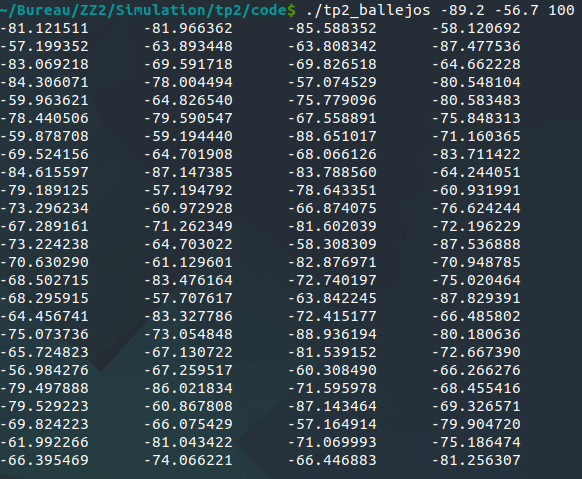
\includegraphics[scale=0.5]{exo2-1.png}
	\caption{Sortie après 100 appels de la fonction $uniform(-89,2,-56,7)$ }    
\end{figure}

\newpage

\section{Exercice 3: Reproduction de tirage aléatoire discret}

Nous allons ici reproduire des distributions discrètes d'abord avec 3 classes puis après plus générale.

\subsection{Simulation discrète avec 3 classes A, B et C}


Pour commencer, j'ai implémenté \textbf{SimulDiscreteABC} qui construit le tableau des probabilités cumulées et observe pour un certain nombre d'itération si nous arrivons à retrouver empiriquement les valeurs attendues.
Le résultat est concluant dès 1000 itérations comme nous pouvons le voir ici

\begin{figure}[H]
\centering
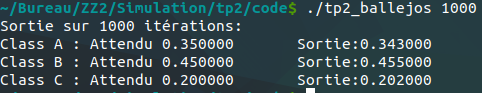
\includegraphics[scale=0.8]{exo3-1.png}
\caption{Sortie de ma fonction $SimulDiscreteABC$ sur 1000 itérations}    
\end{figure}

Plus nous augmentons le nombre de tirage plus le résultat empirique tend vers le résultat théorique ! Ainsi pour 100 000 itérations la sortie est très convaincante.

\begin{figure}[H]
	\centering
	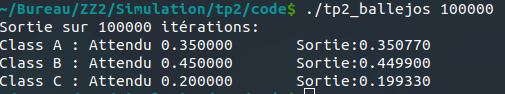
\includegraphics[scale=0.8]{exo3-2.png}
	\caption{Sortie de ma fonction $SimulDiscreteABC$ sur 100000 itérations}    
\end{figure}

\subsection{Simulation discrète avec $n$ classes}

Je me suis inspiré du dernier code que j'ai généralisé. Les différentes étapes de la fonction sont les suivantes: on remplit automatiquement le tableau des probabilités cumulées à l'aide d'un tableau \textbf{proba} passé en argument. On effectue ensuite $n$ nombre de tirage dont le résultat est stocké dans un tableau \textbf{sorti}. Une fois les tirages terminés, on affiche les résultats.

On peut déjà voir que la fonction semble bien fonctionner car nous obtenons les mêmes résultats que la fonction précédente en recréant les 3 classes A, B et C.

\begin{figure}[H]
	\centering
	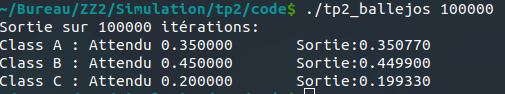
\includegraphics[scale=0.8]{exo3-2.png}
	\caption{Sortie de ma fonction $SimulDiscreteGeneric$ sur 100000 itérations}    
\end{figure}

Maintenant, je me suis amusé à créer un exemple plus poussé pour tester la fonction avec le tableau de proba : \textbf{\{0.5, 0.3, 0.1, 0.05, 0.025, 0.025\}}. Le résultat est très concluant car on arrive à retrouver empiriquement quasiment les mêmes résultats que ceux théorique.

\begin{figure}[H]
	\centering
	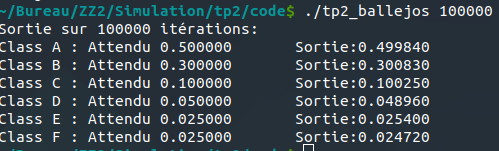
\includegraphics[scale=0.8]{exo3-3.png}
	\caption{Sortie de ma fonction $SimulDiscreteGeneric$ avec 6 classes}    
\end{figure}

Avec 1 000 000 de tirage le résultat empirique tend encore plus vers les probabilités théoriques

\begin{figure}[H]
	\centering
	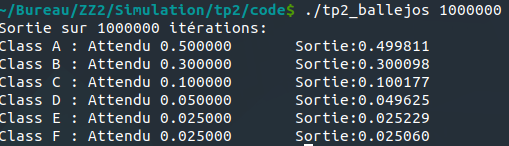
\includegraphics[scale=0.8]{exo3-4.png}
	\caption{Sortie de $SimulDiscreteGeneric$ avec 6 classes et 1000000 de tirages}    
\end{figure}


\section{Exercice 4: Reproduction de tirage aléatoire continu}

Dans cette exercice nous allons reproduire une distribution cette fois-ci continue et cela en inversant la fonction exponentielle.

\subsection{Vérification de la moyenne}

Après avoir implémenté la fonction \textbf{negExp()} qui renvoie des valeurs suivant la fonction $-mean * log(1 - Random)$, j'ai codé en premier temps \textbf{SimulNegExp} qui effectue $n$ tirages aléatoires et vérifie que la moyenne théorique que l'on doit obtenir et la même que celle obtenu empiriquement.

Et voici les résultats pour une moyenne de 11.

\begin{figure}[H]
	\centering
	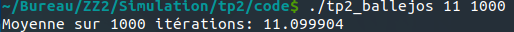
\includegraphics[scale=0.8]{exo4-1.png}
	\caption{Sortie de $SimulNegExp$ avec mean = 11 et 1000 tirages}    
\end{figure}

Dès 1000 tirage le résultat et concluant mais voyons ce qu'il en est avec 1 000 000 de tirage.

\begin{figure}[H]
	\centering
	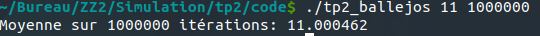
\includegraphics[scale=0.8]{exo4-2.png}
	\caption{Sortie de $SimulNegExp$ avec mean = 11 et 1 000 000 tirages}    
\end{figure}

Le résultat est de plus en plus précis quand on augmente le nombre de tirage !

\subsection{Vérification de la répartition des sorties}

Nous allons maintenant regarder la répartition des sorties aléatoires.

Pour cela j'ai créé une fonction \textbf{DiscretDitribNegExp} qui effectue $n$ tirage aléatoire avec la fonction  \textbf{negExp()} et regarde la répartition des données sur 22 intervalles entre 0 et 22.

Regardons les sorties pour 1000 itérations et la courbe associée:

\begin{figure}[H]
	\centering
	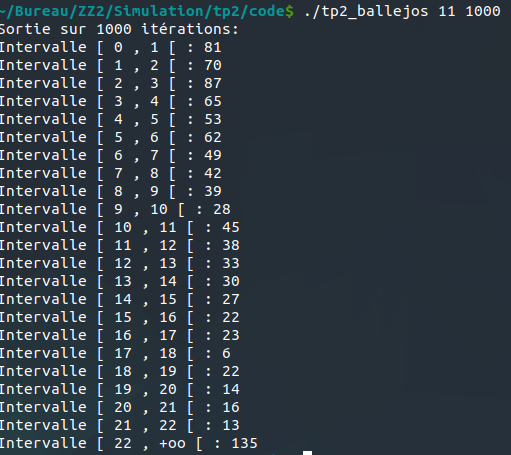
\includegraphics[scale=0.4]{exo4-4.png}
	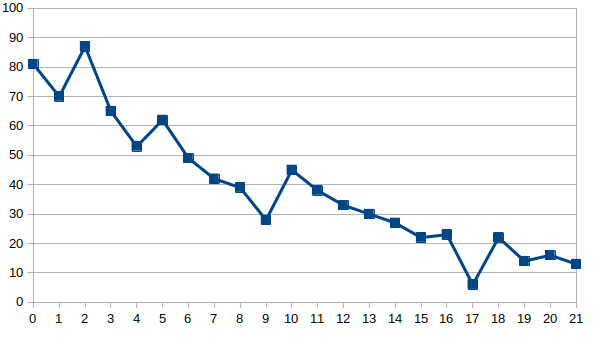
\includegraphics[scale=0.4]{exo4-3.png}
	\caption{Sortie de $DiscretDitribNegExp$ avec mean = 11 et 1000 tirages}    
\end{figure}

La courbe est encore bancale et nous n'arrivons pas à discerner la moyenne, le résultat n'est pas exploitable

Voyons maintenant avec 1 000 000 de tirage:

\begin{figure}[H]
	\centering
	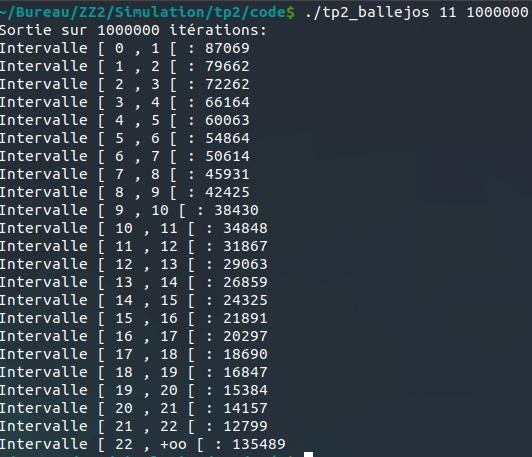
\includegraphics[scale=0.4]{exo4-6.png}
	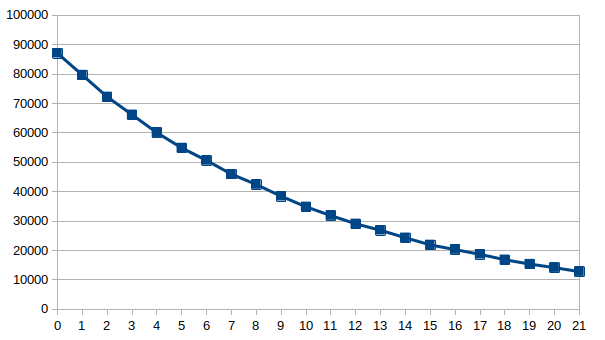
\includegraphics[scale=0.4]{exo4-5.png}
	\caption{Sortie de $DiscretDitribNegExp$ avec mean = 11 et 1 000 000 tirages}    
\end{figure}

Le résultat est déjà beaucoup plus intéressant, on distingue bien la courbe exponentielle négative ayant 11 pour moyenne.

\newpage

\section{Exercice 5: Simulation d'une loi non inversible}

Certaine loi n'ont aujourd'hui toujours pas été inversé et nous allons essayer ici de les reproduire empiriquement.

\subsection{Reproduction de la loi normale avec des lancés de dés}

Après avoir créé une fonction qui simule un lancé de dés (nombre aléatoire entre 1 et 6) j'ai crée la fonction \textbf{SimulDice} qui effectue 30 tirages de dès, additionne les sorties et cela $n$ fois. Grâce à cette expérience nous allons réussir à approcher une courbe gaussienne entre 30 et 180 (qui correspond aux bornes min et max de notre expérience)

Regardons les sorties pour différents nombre de tirage.

\begin{figure}[H]
	\centering
	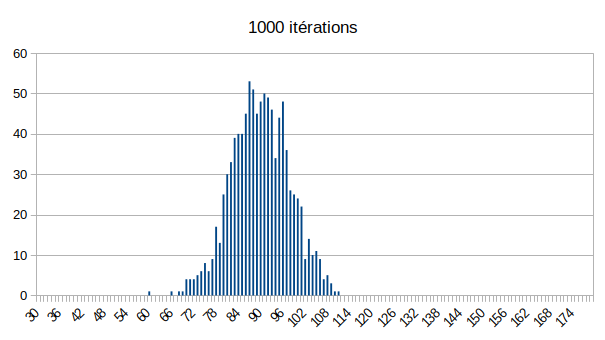
\includegraphics[scale=0.35]{exo5-1.png}
	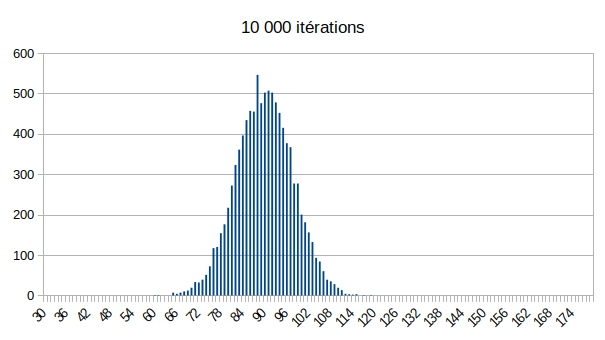
\includegraphics[scale=0.35]{exo5-2.png}
	\caption{Sortie de $SimulDice$ avec 1000 et 10 000 tirages}    
\end{figure}

Ici, on remarque qu'une gaussienne est en train de se créer mais celle-ci n'est pas parfaite. Voyons voir ce que cela donne avec plus d'itérations.

\begin{figure}[H]
	\centering
	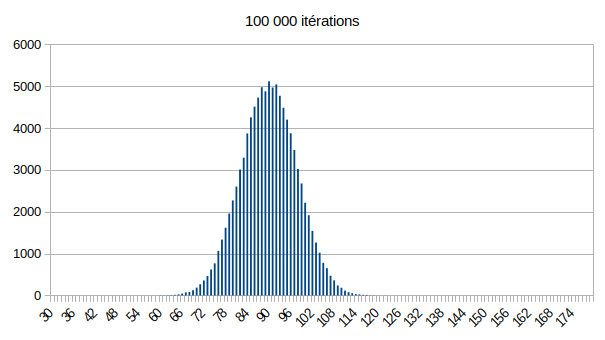
\includegraphics[scale=0.35]{exo5-3.png}
	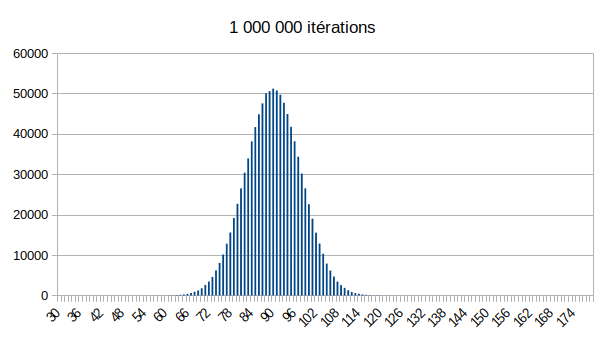
\includegraphics[scale=0.35]{exo5-4.png}
	\caption{Sortie de $SimulDice$ avec 100 000 et 1 000 000 tirages}    
\end{figure}

Avec 100 000 itérations, la courbe n'est pas encore totalement parfaite. Avec 1 000 000, on distingue une gaussienne parfaite. On a donc réussi avec cette expérience de lancé de dés à reproduire une gaussienne. Ceci dit le cout d'exécution est très cher et il faut beaucoup d'itération pour obtenir une très belle courbe. 

Regardons maintenant si il n'est pas possible d'obtenir cette même courbe avec un moyen plus efficace. 

\subsection{Reproduction de la loi normale avec Box and Muller}

Nous allons maintenant reproduire une gaussienne en utilisant le couple d'équation de Box and Muller qui permet à l'aide de deux nombres tirés aléatoirement d'obtenir 2 points de la gaussienne centrée en 0.

J'ai donc implémenté deux fonctions \textbf{BoxAndMullerX1} et \textbf{BoxAndMullerX2} qui renvoie le résultat des équations de Box and Muller en prenant en argument deux nombres supposés tirés aléatoirement.

\begin{figure}[H]
	\centering
	\begin{align}
		x_{1} = \cos(2 \pi Rn_{2})(-2 \ln(Rn_{1}))^{\frac{1}{2}} \\
		x_{1} = \sin(2 \pi Rn_{2})(-2 \ln(Rn_{1}))^{\frac{1}{2}}
	\end{align}
	\caption{Les deux équations de Box and Muller}    
\end{figure}

Ensuite j'ai crée la fonction \textbf{SimulBoxAndMuller} qui prend en argument un nombre d'itération. Elle va faire tirer deux nombres aléatoires et faire appel au deux fonctions de Box and Muller afin de stocker ensuite les sorties.

Afin d'éviter un $if$ à rallonge, j'ai écrit une petite ligne de code permettant de stocker les résultats sur des intervalles de 0.5 (par exemple $[-5 , -4.5]$) dans un tableau de taille 20.

La voici:

\begin{lstlisting}{C}
	// Réajustement sur un tableau de taille 20 entre 0 et 19 (* 10 + 50 / 5)
	repartition[(int)((BoxAndMullerX1(u1, u2) * 10 + 50) / 5)]++;
	repartition[(int)((BoxAndMullerX2(u1, u2) * 10 + 50) / 5)]++;
\end{lstlisting}

\bigskip

Au final voici la sortie obtenu tout d'abord avec seulement 1000 itérations puis avec 1 000 000.

\begin{figure}[H]
	\centering
	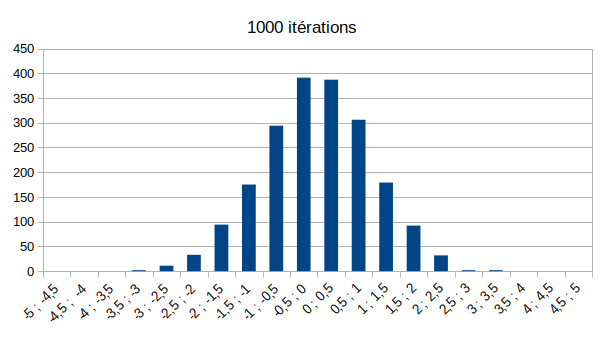
\includegraphics[scale=0.35]{exo5-5.png}
	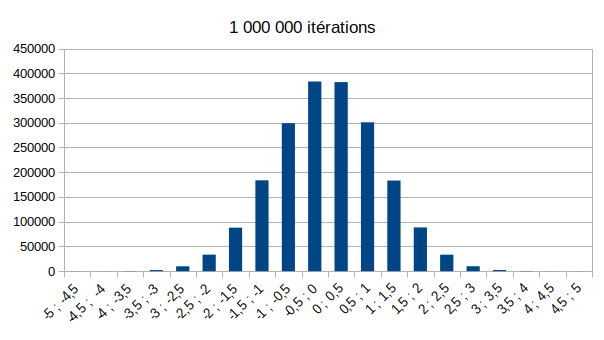
\includegraphics[scale=0.35]{exo5-6.png}
	\caption{Sortie de $SimulBoxAndMuller$ avec 1000 et 1 000 000 tirages}    
\end{figure}

On remarque qu'avec 1000 itérations la gaussienne est quasi parfaite ! On a donc trouver une méthode bien plus efficace et rapide pour simuler empiriquement une courbe gaussienne.

J'ai tout de même aussi représenter la courbe pour 1 000 000 d'itérations et on remarque qu'a part sur le milieu de l'échantillon le résultat et quasiment le même.

\section{Exercice 6: Les librairies}

En C/C++, la bibliothèque qui semblent pouvoir effectuer tout ce que l'on a fait précédemment est \textbf{Boost Random Number Library Distributions}. Toutes les informations sont disponible sur le site de la librairie que vous pouvez trouver en cliquant \href{https://www.boost.org/doc/libs/1_39_0/libs/random/}{\underline{ici}}.

\bigskip

En Java, \textbf{The Apache Commons Mathematics Library} semble posséder toutes les méthodes nécessaires permettant de faire ce que l'on a fait durant le TP. Cette bibliothèque possède par exemple la méthode $NormalDistribution$. Le site de la librairie ce trouve \href{https://commons.apache.org/proper/commons-math/javadocs/api-3.6.1/index.html?org/apache/commons/math3/random/class-use/RandomGenerator.html}{\underline{ici}}..

\section{Fonctions "Outil"}

Pour m'aider lors de mon travail j'ai codé deux fonctions annexes dont je vais prendre quelques lignes pour expliquer leur but.

La première est la fonction \textbf{exportData} qui reçoit un tableau ainsi que la taille de celui-ci et une chaine de caractère.
Elle permet d'exporter les données de sortie du tableau dans un fichier formaté qui est facilement manipulable sur Excel ou LibreOffice Calc.

La seconde est \textbf{afficheHistogramme} qui permet d'afficher dans mon terminal une pré visualisation très basique de l'histogramme des données stockés dans un tableau.

La fonction à l'aide de \textbf{valeurMax} va automatiquement trouver la donnée la plus grande afin de représenter proprement l'histogramme.

\begin{figure}[H]
	\centering
	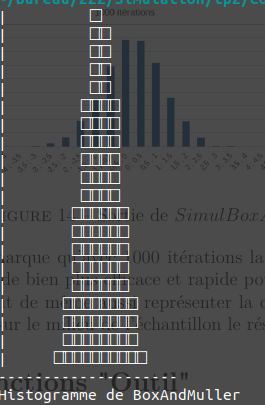
\includegraphics[scale=0.35]{outil-1.png}
	\caption{Exemple d'histogramme généré par ma fonction}    
\end{figure}


\listoffigures

\end{document}


